\documentclass [a4paper] {article}
\usepackage[utf8]{inputenc}
\title{PRÁCTICA 2 FUNDAMENTOS DE LA CIENCIA DE DATOS}
\author{Javier Martín Gómez, Ignacio Afuera Díaz, Laura Gil Gómez, & Christian Ayala Urbanos}
\usepackage{Sweave}
\begin{document}
\maketitle

\begin{abstract}
En esta práctica hemos realizado un análisis de asociación de datos con R. Para ello,
hemos utilizado el algoritmo de asociación de datos visto en clase, el algoritmo
apriori. Además, hemos utilizado otro extra, llamado eclat. Para poder usar estos
algoritmos hemos tenido que instalar el paquete y librería arules, y para su
la visualización de las asociaciones, hemos utilizado arulesViz.

\end{abstract}

\newpage
\tableofcontents
\newpage


\section{Análisis de asociación cesta compra }
En esta sección, vamos a realizar el análisis de asociación del ejercicio realizado
en clase. Primero, hemos utilizado el algoritmo apriori (visto en clase) y después,
hemos utilizado una alternativa a dicho algoritmo llamada eclat.
\subsection{Pasos iniciales}
Lo primero antes de realizar cualquier algoritmo hay que cargar los datos, en este
primer ejercicio la realizaremos directamente desde el código:

\begin{Schunk}
\begin{Sinput}
> muestra<-Matrix(c(1,1,0,1,1, 1,1,1,1,0, 1,1,0,1,0,1,0,1,1,0, 
+ 1,1,0,0,0, 0,0,0,1,0),6,5,byrow=TRUE,dimnames=list(
+ c("Suceso1","Suceso2","Suceso3","Suceso4","Suceso5","Suceso6"),
+ c("Pan","Agua","Cafe","Leche","Naranjas")),sparse=TRUE)
\end{Sinput}
\end{Schunk}

Quedaría la siguiente matriz:

\begin{Schunk}
\begin{Sinput}
> muestra
\end{Sinput}
\begin{Soutput}
6 x 5 sparse Matrix of class "dgCMatrix"
        Pan Agua Cafe Leche Naranjas
Suceso1   1    1    .     1        1
Suceso2   1    1    1     1        .
Suceso3   1    1    .     1        .
Suceso4   1    .    1     1        .
Suceso5   1    1    .     .        .
Suceso6   .    .    .     1        .
\end{Soutput}
\end{Schunk}

Tambien hay que cargar la librería usada:

\begin{Schunk}
\begin{Sinput}
> library(arules)
\end{Sinput}
\end{Schunk}

\subsection{Asociación}
Ahora realizamos las siguientes operaciones para adaptar la matriz a la función
que se va a utilizar en el siguiente paso: construimos una matriz nsparse y 
la transponemos:

\begin{Schunk}
\begin{Sinput}
> muestrangCMatrix<-as(muestra,"nsparseMatrix")
> muestrangCMatrix
\end{Sinput}
\begin{Soutput}
6 x 5 sparse Matrix of class "ngCMatrix"
        Pan Agua Cafe Leche Naranjas
Suceso1   |    |    .     |        |
Suceso2   |    |    |     |        .
Suceso3   |    |    .     |        .
Suceso4   |    .    |     |        .
Suceso5   |    |    .     .        .
Suceso6   .    .    .     |        .
\end{Soutput}
\begin{Sinput}
> transpmuestratrangCMatrix<-t(muestrangCMatrix)
> transpmuestratrangCMatrix
\end{Sinput}
\begin{Soutput}
5 x 6 sparse Matrix of class "ngCMatrix"
         Suceso1 Suceso2 Suceso3 Suceso4 Suceso5 Suceso6
Pan            |       |       |       |       |       .
Agua           |       |       |       .       |       .
Cafe           .       |       .       |       .       .
Leche          |       |       |       |       .       |
Naranjas       |       .       .       .       .       .
\end{Soutput}
\end{Schunk}
A continuación, se obtendrán las transacciones a partir de la matriz mostrada anteriormente y un resumen de ellas:

\begin{Schunk}
\begin{Sinput}
> transacciones<-as(transpmuestratrangCMatrix,"transactions")
> inspect(transacciones)
\end{Sinput}
\begin{Soutput}
    items                     itemsetID
[1] {Pan,Agua,Leche,Naranjas} Suceso1  
[2] {Pan,Agua,Cafe,Leche}     Suceso2  
[3] {Pan,Agua,Leche}          Suceso3  
[4] {Pan,Cafe,Leche}          Suceso4  
[5] {Pan,Agua}                Suceso5  
[6] {Leche}                   Suceso6  
\end{Soutput}
\begin{Sinput}
> summary(transacciones)
\end{Sinput}
\begin{Soutput}
transactions as itemMatrix in sparse format with
 6 rows (elements/itemsets/transactions) and
 5 columns (items) and a density of 0.5666667 

most frequent items:
     Pan    Leche     Agua     Cafe Naranjas  (Other) 
       5        5        4        2        1        0 

element (itemset/transaction) length distribution:
sizes
1 2 3 4 
1 1 2 2 

   Min. 1st Qu.  Median    Mean 3rd Qu.    Max. 
  1.000   2.250   3.000   2.833   3.750   4.000 

includes extended item information - examples:
  labels
1    Pan
2   Agua
3   Cafe

includes extended transaction information - examples:
  itemsetID
1   Suceso1
2   Suceso2
3   Suceso3
\end{Soutput}
\end{Schunk}

\subsubsection{Apriori}
Finalmente, obtendremos las asociaciones de la matriz que hemos cargado anteriormente a través del algoritmo apriori
con soporte 0.5 y confianza 0.8 para este caso.

\begin{Schunk}
\begin{Sinput}
> asociacionesap<-apriori(transacciones,parameter=list(support=0.5,confidence=0.8))
\end{Sinput}
\begin{Soutput}
Apriori

Parameter specification:
 confidence minval smax arem  aval originalSupport maxtime support minlen
        0.8    0.1    1 none FALSE            TRUE       5     0.5      1
 maxlen target  ext
     10  rules TRUE

Algorithmic control:
 filter tree heap memopt load sort verbose
    0.1 TRUE TRUE  FALSE TRUE    2    TRUE

Absolute minimum support count: 3 

set item appearances ...[0 item(s)] done [0.00s].
set transactions ...[5 item(s), 6 transaction(s)] done [0.00s].
sorting and recoding items ... [3 item(s)] done [0.00s].
creating transaction tree ... done [0.00s].
checking subsets of size 1 2 3 done [0.03s].
writing ... [7 rule(s)] done [0.00s].
creating S4 object  ... done [0.00s].
\end{Soutput}
\begin{Sinput}
> inspect(asociacionesap)
\end{Sinput}
\begin{Soutput}
    lhs             rhs     support   confidence coverage  lift count
[1] {}           => {Leche} 0.8333333 0.8333333  1.0000000 1.00 5    
[2] {}           => {Pan}   0.8333333 0.8333333  1.0000000 1.00 5    
[3] {Agua}       => {Pan}   0.6666667 1.0000000  0.6666667 1.20 4    
[4] {Pan}        => {Agua}  0.6666667 0.8000000  0.8333333 1.20 4    
[5] {Leche}      => {Pan}   0.6666667 0.8000000  0.8333333 0.96 4    
[6] {Pan}        => {Leche} 0.6666667 0.8000000  0.8333333 0.96 4    
[7] {Agua,Leche} => {Pan}   0.5000000 1.0000000  0.5000000 1.20 3    
\end{Soutput}
\end{Schunk}

\subsubsection{Eclat}
El algoritmo Apriori no es perfecto y han aparecido algunos algoritmos basados en
árboles para superar las dificultades presentadas por Apriori. Uno de ellos es Eclat, el cual combina la búsqueda en profundidad con una lista de todos los
identificadores de las transacciones.

Ahora lo aplicaremos en el ejemplo de la cesta de la compra, para ello haremos uso de dos funciones: eclat y ruleInduction. Antes de aplicar estas funciones, debemos obtener las transacciones de la misma manera que se vio en el algoritmo Apriori.

En primer lugar usamos la función eclat, aqui especificamos unícamente el soporte (supp=0.5).
\begin{Schunk}
\begin{Sinput}
> itemsets <- eclat(transacciones, parameter = list(supp = 0.5, maxlen = 5))
\end{Sinput}
\begin{Soutput}
Eclat

parameter specification:
 tidLists support minlen maxlen            target  ext
    FALSE     0.5      1      5 frequent itemsets TRUE

algorithmic control:
 sparse sort verbose
      7   -2    TRUE

Absolute minimum support count: 3 

create itemset ... 
set transactions ...[5 item(s), 6 transaction(s)] done [0.00s].
sorting and recoding items ... [3 item(s)] done [0.00s].
creating bit matrix ... [3 row(s), 6 column(s)] done [0.00s].
writing  ... [7 set(s)] done [0.00s].
Creating S4 object  ... done [0.00s].
\end{Soutput}
\end{Schunk}

En segundo lugar usamos la función ruleInduction, donde se indica la confianza
y las transacciones (confidence = 0.8):
\begin{Schunk}
\begin{Sinput}
> rules <- ruleInduction(itemsets, transacciones, confidence = 0.8)
> inspect(rules)
\end{Sinput}
\begin{Soutput}
    lhs             rhs     support   confidence lift itemset
[1] {Agua,Leche} => {Pan}   0.5000000 1.0        1.20 1      
[2] {Agua}       => {Pan}   0.6666667 1.0        1.20 2      
[3] {Pan}        => {Agua}  0.6666667 0.8        1.20 2      
[4] {Leche}      => {Pan}   0.6666667 0.8        0.96 4      
[5] {Pan}        => {Leche} 0.6666667 0.8        0.96 4      
\end{Soutput}
\end{Schunk}

\newpage
\subsubsection{Representación gráfica de Apriori}
A continuación, vamos a representar los resultados obtenidos anteriormente en forma de gráfica. Para ello llamamos a la función plot usando la librería aRulesViz.
Se representa un grafo dirigido en el que se ven las asociaciones:
\newline
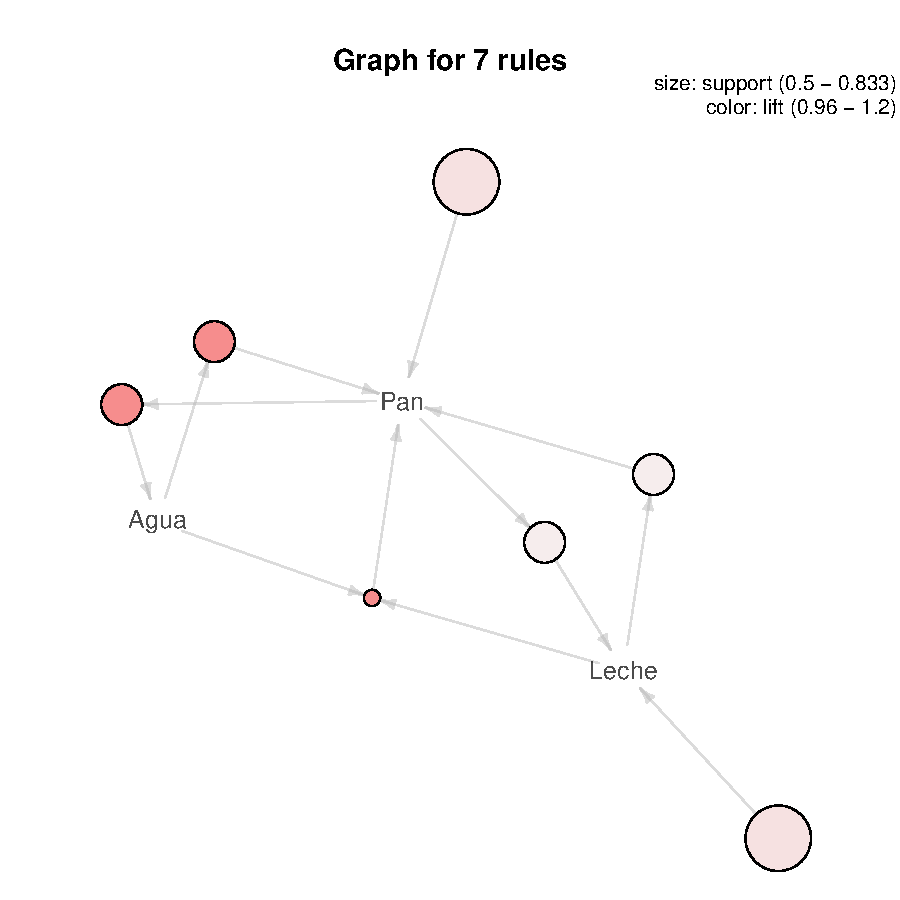
\includegraphics{Memoria-Figura 1}
\newline
Ahora mostramos la gráfica en forma de puntos dispersos. Cada uno de los puntos representa una asociación.
\newline
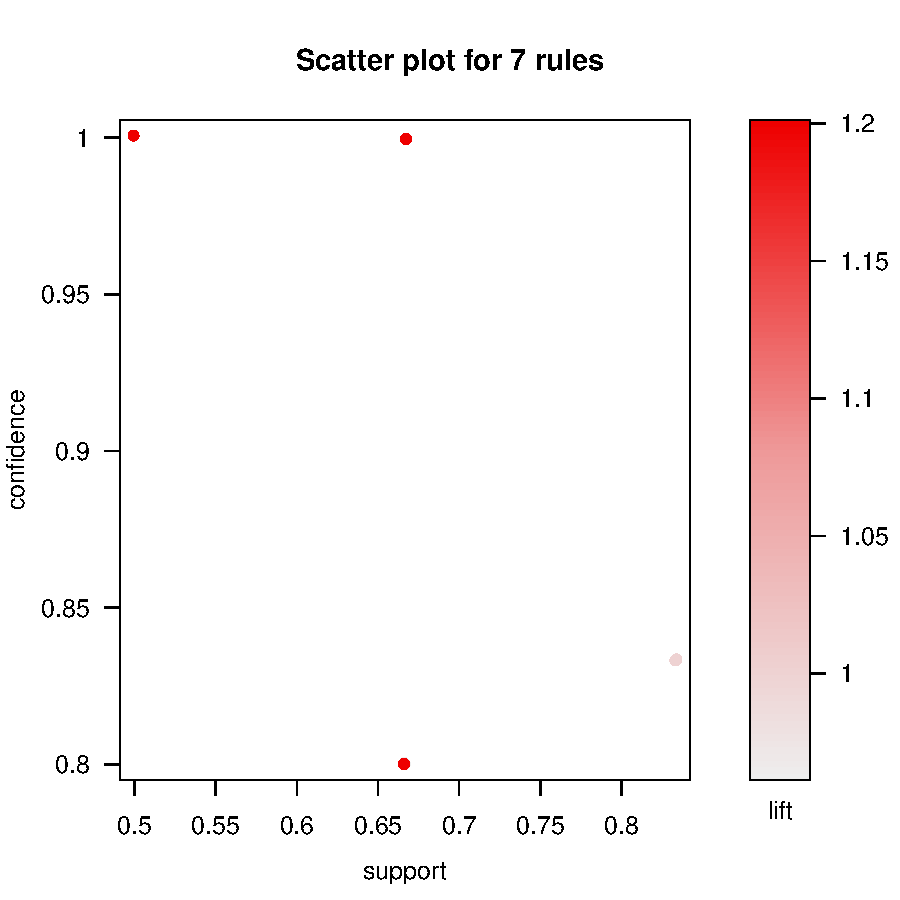
\includegraphics{Memoria-Figura 2}
\subsubsection{Representación gráfica de Eclat}

Hacemos lo mismo para representar los datos obtenidos con el algoritmo Eclat.
\newline
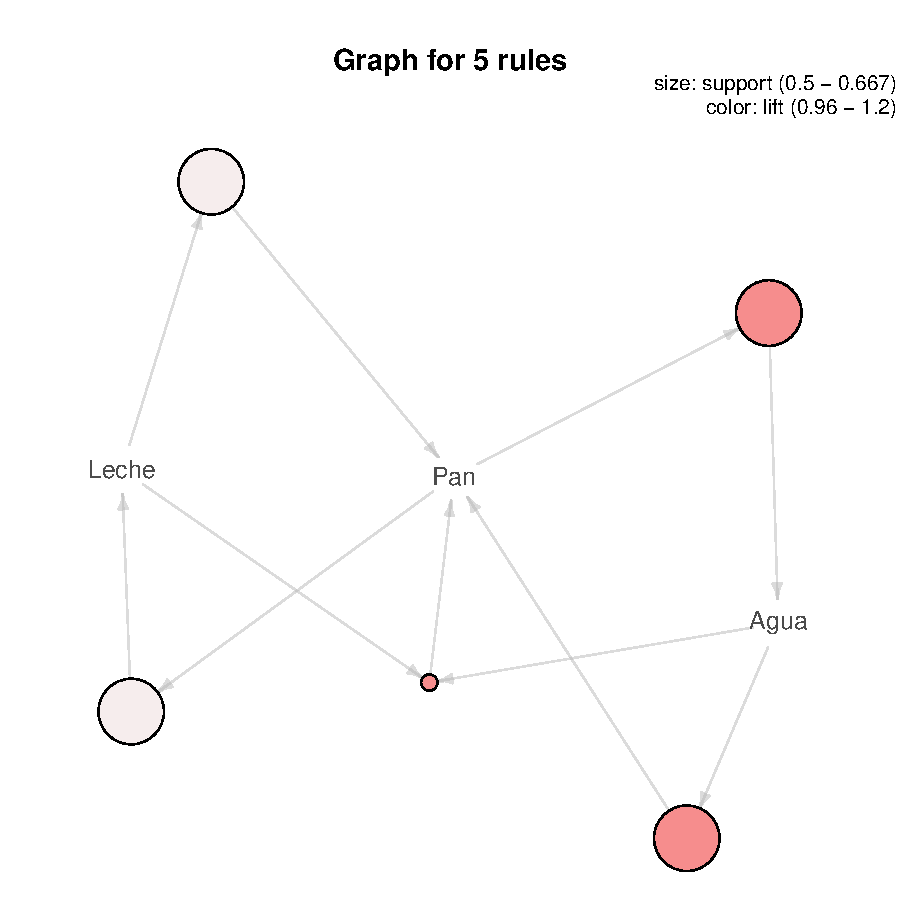
\includegraphics{Memoria-Figura 3}
\newline
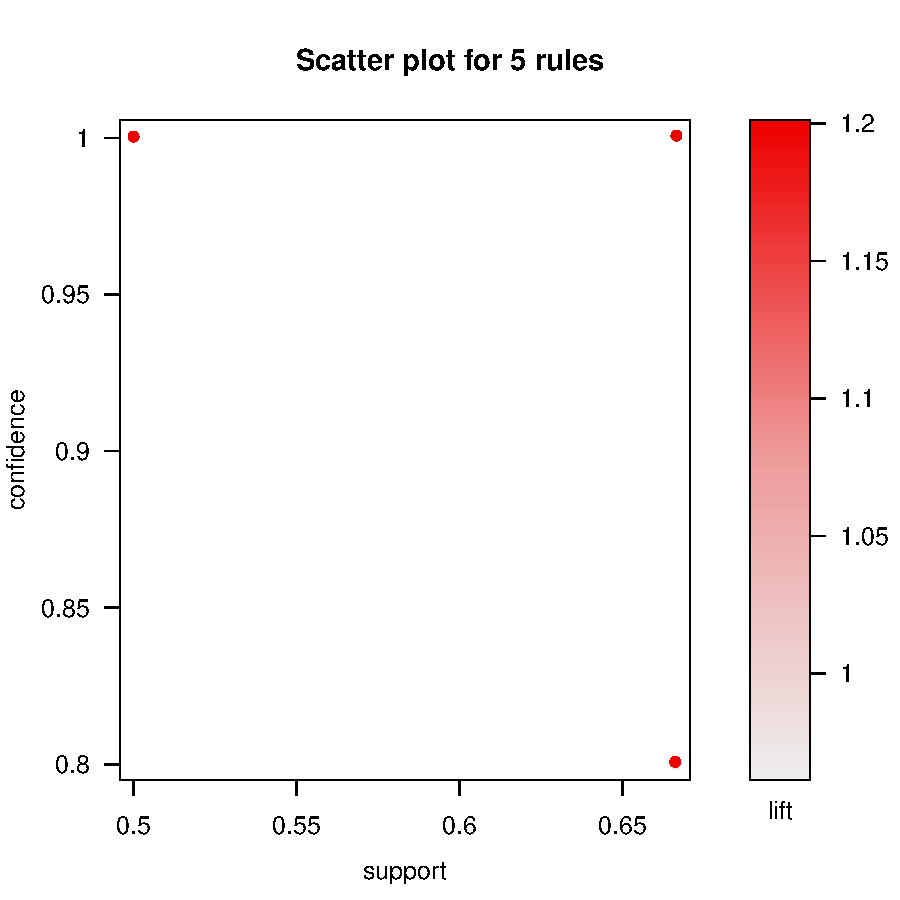
\includegraphics{Memoria-Figura 4}

\section{Análisis de asociación compra de ropa }
En esta sección, vamos a analizar la asociación de diferentes compras de prendas de ropa.
Al igual que en el apartado anterior, vamos a utilizar los algoritmos apriori y eclat,
con la diferencia de que ahora vamos a leer los datos de un archivo Excel y de un archivo
txt.

\subsection{Lectura datos Excel}
Para leer los datos del archivo Excel, primero tenemos que instalar los paquetes
y librerías necesarios

\begin{Schunk}
\begin{Sinput}
> install.packages("pastecs")
> install.packages("xlsx")
> library(pastecs)
> library(xlsx)
\end{Sinput}
\end{Schunk}

Ahora, leemos los datos del archivo Excel y los visualizamos en forma de matriz:

\begin{Schunk}
\begin{Sinput}
> datosExcel<-Matrix(as.matrix(read.xlsx("ropa.xlsx", 1)),byrow=TRUE, sparse=TRUE )
> datosExcel
\end{Sinput}
\begin{Soutput}
9 x 9 sparse Matrix of class "dgCMatrix"
      Camisetas Vaqueros Zapatos Sneakers Abrigos Calcetines Sudaderas
 [1,]         1        1       .        1       .          .         1
 [2,]         .        .       1        .       .          1         1
 [3,]         .        1       1        .       1          1         1
 [4,]         1        .       1        1       .          1         .
 [5,]         .        1       1        1       1          1         1
 [6,]         .        .       .        1       .          1         .
 [7,]         1        1       .        1       .          .         1
 [8,]         .        1       .        1       1          .         1
 [9,]         1        1       1        .       .          1         .
      Calzoncillos Camisa.
 [1,]            .       .
 [2,]            1       .
 [3,]            .       .
 [4,]            .       1
 [5,]            .       .
 [6,]            1       1
 [7,]            .       .
 [8,]            .       .
 [9,]            .       1
\end{Soutput}
\end{Schunk}

\subsection{Asociación desde el archivo Excel}
Para realizar la asociación, tenemos que adaptar la matriz a la función
que se va a utilizar en el siguiente paso. A continuación, construimos la matriz nparse
y la trasponemos:

\begin{Schunk}
\begin{Sinput}
> datosExcelngCMatrix<-as(datosExcel,"nsparseMatrix")
> datosExcelngCMatrix
\end{Sinput}
\begin{Soutput}
9 x 9 sparse Matrix of class "ngCMatrix"
      Camisetas Vaqueros Zapatos Sneakers Abrigos Calcetines Sudaderas
 [1,]         |        |       .        |       .          .         |
 [2,]         .        .       |        .       .          |         |
 [3,]         .        |       |        .       |          |         |
 [4,]         |        .       |        |       .          |         .
 [5,]         .        |       |        |       |          |         |
 [6,]         .        .       .        |       .          |         .
 [7,]         |        |       .        |       .          .         |
 [8,]         .        |       .        |       |          .         |
 [9,]         |        |       |        .       .          |         .
      Calzoncillos Camisa.
 [1,]            .       .
 [2,]            |       .
 [3,]            .       .
 [4,]            .       |
 [5,]            .       .
 [6,]            |       |
 [7,]            .       .
 [8,]            .       .
 [9,]            .       |
\end{Soutput}
\begin{Sinput}
> trspDatosExcelngCMatrix<-t(datosExcelngCMatrix)
> trspDatosExcelngCMatrix
\end{Sinput}
\begin{Soutput}
9 x 9 sparse Matrix of class "ngCMatrix"
                              
Camisetas    | . . | . . | . |
Vaqueros     | . | . | . | | |
Zapatos      . | | | | . . . |
Sneakers     | . . | | | | | .
Abrigos      . . | . | . . | .
Calcetines   . | | | | | . . |
Sudaderas    | | | . | . | | .
Calzoncillos . | . . . | . . .
Camisa.      . . . | . | . . |
\end{Soutput}
\end{Schunk}

Obtenemos la transacciones a partir de la matriz anterior y un resumen de ellas:

\begin{Schunk}
\begin{Sinput}
> transaccionesTxt<-as(trspDatosTxtngCMatrix,"transactions")
> summary(transaccionesTxt)
\end{Sinput}
\begin{Soutput}
transactions as itemMatrix in sparse format with
 9 rows (elements/itemsets/transactions) and
 9 columns (items) and a density of 0.5061728 

most frequent items:
  Vaqueros   Sneakers Calcetines  Sudaderas    Zapatos    (Other) 
         6          6          6          6          5         12 

element (itemset/transaction) length distribution:
sizes
4 5 6 
5 3 1 

   Min. 1st Qu.  Median    Mean 3rd Qu.    Max. 
  4.000   4.000   4.000   4.556   5.000   6.000 

includes extended item information - examples:
     labels
1 Camisetas
2  Vaqueros
3   Zapatos

includes extended transaction information - examples:
  itemsetID
1         1
2         2
3         3
\end{Soutput}
\end{Schunk}

\subsubsection{Apriori desde el archivo Excel}
Por último, hallamos las asociaciones de la matriz cargada a través del algoritmo
apriori con un soporte 0.5 y confianza 0.8:

\begin{Schunk}
\begin{Sinput}
> asociacionesExcel<-apriori(transaccionesExcel, 
+ parameter=list(support=0.5, confidence=0.8))
\end{Sinput}
\begin{Soutput}
Apriori

Parameter specification:
 confidence minval smax arem  aval originalSupport maxtime support minlen
        0.8    0.1    1 none FALSE            TRUE       5     0.5      1
 maxlen target  ext
     10  rules TRUE

Algorithmic control:
 filter tree heap memopt load sort verbose
    0.1 TRUE TRUE  FALSE TRUE    2    TRUE

Absolute minimum support count: 4 

set item appearances ...[0 item(s)] done [0.00s].
set transactions ...[9 item(s), 9 transaction(s)] done [0.00s].
sorting and recoding items ... [5 item(s)] done [0.00s].
creating transaction tree ... done [0.00s].
checking subsets of size 1 2 done [0.00s].
writing ... [4 rule(s)] done [0.00s].
creating S4 object  ... done [0.00s].
\end{Soutput}
\begin{Sinput}
> inspect(asociacionesExcel)
\end{Sinput}
\begin{Soutput}
    lhs             rhs          support   confidence coverage  lift count
[1] {Zapatos}    => {Calcetines} 0.5555556 1.0000000  0.5555556 1.50 5    
[2] {Calcetines} => {Zapatos}    0.5555556 0.8333333  0.6666667 1.50 5    
[3] {Sudaderas}  => {Vaqueros}   0.5555556 0.8333333  0.6666667 1.25 5    
[4] {Vaqueros}   => {Sudaderas}  0.5555556 0.8333333  0.6666667 1.25 5    
\end{Soutput}
\end{Schunk}

\subsection{Lectura datos txt}
Para leer los datos del archivo txt, únicamente tenemos que usar la función read.table:


\begin{Schunk}
\begin{Sinput}
> datostxt<-Matrix(as.matrix(read.table("ropa.txt")),byrow=TRUE, sparse=TRUE )
> datostxt
\end{Sinput}
\begin{Soutput}
9 x 9 sparse Matrix of class "dgCMatrix"
  Camisetas Vaqueros Zapatos Sneakers Abrigos Calcetines Sudaderas Calzoncillos
1         1        1       .        1       .          .         1            .
2         .        .       1        .       .          1         1            1
3         .        1       1        .       1          1         1            .
4         1        .       1        1       .          1         .            .
5         .        1       1        1       1          1         1            .
6         .        .       .        1       .          1         .            1
7         1        1       .        1       .          .         1            .
8         .        1       .        1       1          .         1            .
9         1        1       1        .       .          1         .            .
  Camisa
1      .
2      .
3      .
4      1
5      .
6      1
7      .
8      .
9      1
\end{Soutput}
\end{Schunk}

\subsection{Asociación desde el archivo txt}
Para realizar la asociación, tenemos que adaptar la matriz a la función
que se va a utilizar en el siguiente paso. A continuación, construimos la matriz nparse
y la trasponemos:

\begin{Schunk}
\begin{Sinput}
> datosTxtngCMatrix<-as(datostxt,"nsparseMatrix")
> datosTxtngCMatrix
\end{Sinput}
\begin{Soutput}
9 x 9 sparse Matrix of class "ngCMatrix"
  Camisetas Vaqueros Zapatos Sneakers Abrigos Calcetines Sudaderas Calzoncillos
1         |        |       .        |       .          .         |            .
2         .        .       |        .       .          |         |            |
3         .        |       |        .       |          |         |            .
4         |        .       |        |       .          |         .            .
5         .        |       |        |       |          |         |            .
6         .        .       .        |       .          |         .            |
7         |        |       .        |       .          .         |            .
8         .        |       .        |       |          .         |            .
9         |        |       |        .       .          |         .            .
  Camisa
1      .
2      .
3      .
4      |
5      .
6      |
7      .
8      .
9      |
\end{Soutput}
\begin{Sinput}
> trspDatosTxtngCMatrix<-t(datosTxtngCMatrix)
> trspDatosTxtngCMatrix
\end{Sinput}
\begin{Soutput}
9 x 9 sparse Matrix of class "ngCMatrix"
             1 2 3 4 5 6 7 8 9
Camisetas    | . . | . . | . |
Vaqueros     | . | . | . | | |
Zapatos      . | | | | . . . |
Sneakers     | . . | | | | | .
Abrigos      . . | . | . . | .
Calcetines   . | | | | | . . |
Sudaderas    | | | . | . | | .
Calzoncillos . | . . . | . . .
Camisa       . . . | . | . . |
\end{Soutput}
\end{Schunk}

Ahora, obtenemos las transacciones a partir de la matriz anterior junto a su resumen:


\begin{Schunk}
\begin{Sinput}
> transaccionesTxt<-as(trspDatosTxtngCMatrix,"transactions")
> summary(transaccionesTxt)
\end{Sinput}
\begin{Soutput}
transactions as itemMatrix in sparse format with
 9 rows (elements/itemsets/transactions) and
 9 columns (items) and a density of 0.5061728 

most frequent items:
  Vaqueros   Sneakers Calcetines  Sudaderas    Zapatos    (Other) 
         6          6          6          6          5         12 

element (itemset/transaction) length distribution:
sizes
4 5 6 
5 3 1 

   Min. 1st Qu.  Median    Mean 3rd Qu.    Max. 
  4.000   4.000   4.000   4.556   5.000   6.000 

includes extended item information - examples:
     labels
1 Camisetas
2  Vaqueros
3   Zapatos

includes extended transaction information - examples:
  itemsetID
1         1
2         2
3         3
\end{Soutput}
\end{Schunk}


\subsubsection{Apriori desde el archivo txt}
Para terminar, obtenemos las asociaciones de la matriz con los datos de la ropa
con soporte 0.4 y confianza 0.7:

\begin{Schunk}
\begin{Sinput}
> asociacionesTxt<-apriori(transaccionesTxt, parameter=list(support=0.4, confidence=0.7))
\end{Sinput}
\begin{Soutput}
Apriori

Parameter specification:
 confidence minval smax arem  aval originalSupport maxtime support minlen
        0.7    0.1    1 none FALSE            TRUE       5     0.4      1
 maxlen target  ext
     10  rules TRUE

Algorithmic control:
 filter tree heap memopt load sort verbose
    0.1 TRUE TRUE  FALSE TRUE    2    TRUE

Absolute minimum support count: 3 

set item appearances ...[0 item(s)] done [0.00s].
set transactions ...[9 item(s), 9 transaction(s)] done [0.00s].
sorting and recoding items ... [6 item(s)] done [0.00s].
creating transaction tree ... done [0.00s].
checking subsets of size 1 2 3 done [0.00s].
writing ... [7 rule(s)] done [0.00s].
creating S4 object  ... done [0.00s].
\end{Soutput}
\begin{Sinput}
> inspect(asociacionesTxt)
\end{Sinput}
\begin{Soutput}
    lhs                     rhs          support   confidence coverage  lift
[1] {Zapatos}            => {Calcetines} 0.5555556 1.0000000  0.5555556 1.50
[2] {Calcetines}         => {Zapatos}    0.5555556 0.8333333  0.6666667 1.50
[3] {Sudaderas}          => {Vaqueros}   0.5555556 0.8333333  0.6666667 1.25
[4] {Vaqueros}           => {Sudaderas}  0.5555556 0.8333333  0.6666667 1.25
[5] {Sneakers,Sudaderas} => {Vaqueros}   0.4444444 1.0000000  0.4444444 1.50
[6] {Vaqueros,Sneakers}  => {Sudaderas}  0.4444444 1.0000000  0.4444444 1.50
[7] {Vaqueros,Sudaderas} => {Sneakers}   0.4444444 0.8000000  0.5555556 1.20
    count
[1] 5    
[2] 5    
[3] 5    
[4] 5    
[5] 4    
[6] 4    
[7] 4    
\end{Soutput}
\end{Schunk}


\subsubsection{Eclat}
El agoritmo Eclat es una alternativa a apriori, como hemos explicado anteriormente.
Para poder usarlo y hallar las asociaciones, primero tenemos que usar la función eclat
donde especificamos el soporte 0.5. Solo vamos a hacerlo del archivo txt, ya que los datos
son los mismos que en el Excel:

\begin{Schunk}
\begin{Sinput}
> itemsets <- eclat(transaccionesExcel,
+ 		parameter = list(supp = 0.5, maxlen = 5))
\end{Sinput}
\begin{Soutput}
Eclat

parameter specification:
 tidLists support minlen maxlen            target  ext
    FALSE     0.5      1      5 frequent itemsets TRUE

algorithmic control:
 sparse sort verbose
      7   -2    TRUE

Absolute minimum support count: 4 

create itemset ... 
set transactions ...[9 item(s), 9 transaction(s)] done [0.00s].
sorting and recoding items ... [5 item(s)] done [0.00s].
creating bit matrix ... [5 row(s), 9 column(s)] done [0.00s].
writing  ... [7 set(s)] done [0.00s].
Creating S4 object  ... done [0.00s].
\end{Soutput}
\end{Schunk}

Ahora, usamos ruleInduction, donde indicamos la confianza 0.8 y podemos ver
las transacciones:

\begin{Schunk}
\begin{Sinput}
> rules <- ruleInduction(itemsets, transaccionesExcel, confidence = 0.8)
> inspect(rules)
\end{Sinput}
\begin{Soutput}
    lhs             rhs          support   confidence lift itemset
[1] {Calcetines} => {Zapatos}    0.5555556 0.8333333  1.50 1      
[2] {Zapatos}    => {Calcetines} 0.5555556 1.0000000  1.50 1      
[3] {Sudaderas}  => {Vaqueros}   0.5555556 0.8333333  1.25 2      
[4] {Vaqueros}   => {Sudaderas}  0.5555556 0.8333333  1.25 2      
\end{Soutput}
\end{Schunk}


\subsubsection{Representación gráfica de Apriori}
A continuación, vamos a visualizar los datos obtenidos anteriormente con apriori. Para ello
utilizamos la librería arulesViz. Primero representamos un grafo dirigido donde podemos ver
las asociaciones:


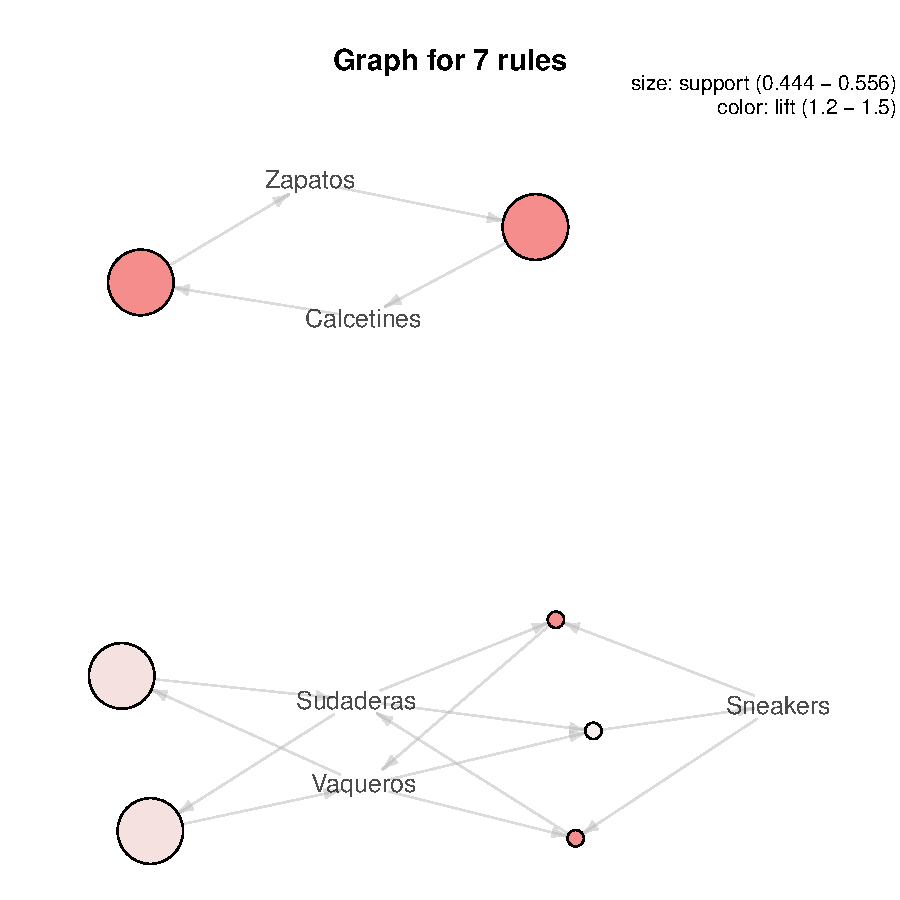
\includegraphics{Memoria-Figura 5}

Ahora, visualizamos la gráfica de puntos dispersos, donde 
cada punto representa una asociación:
\newline
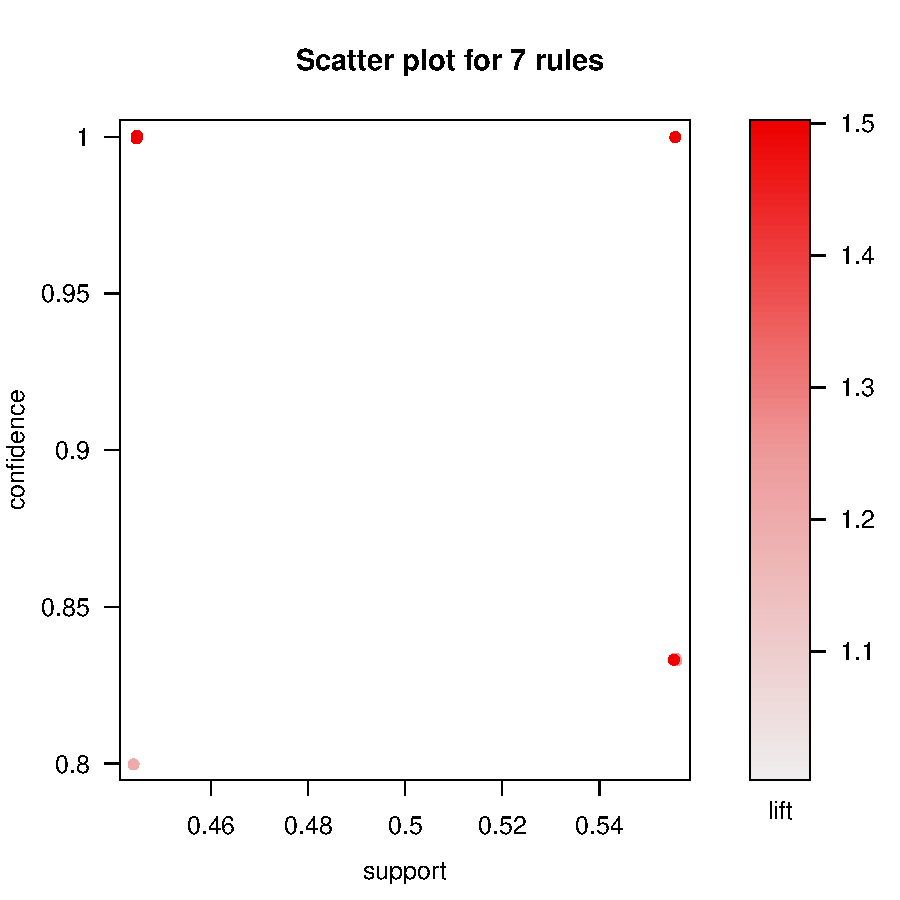
\includegraphics{Memoria-Figura 6}

\subsubsection{Representación gráfica de Eclat}
Volvemos a representar el grafo y la gráfica de puntos dispersos, pero ahora
con los datos obtenidos del algoritmo Eclat:

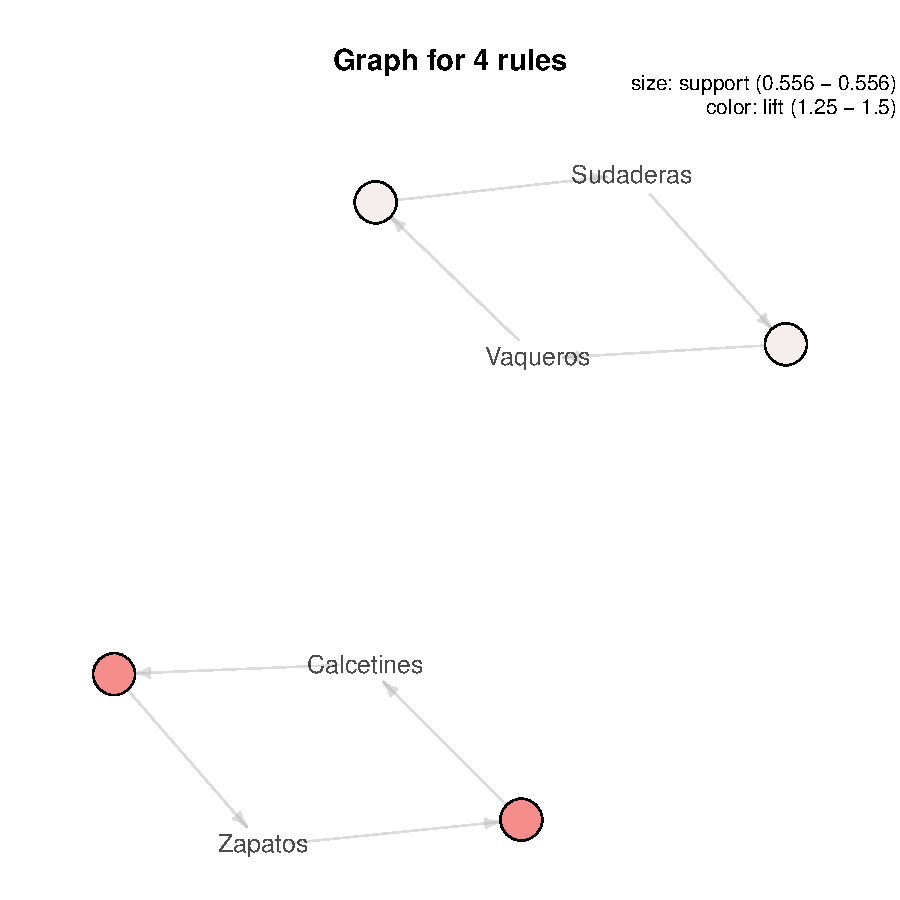
\includegraphics{Memoria-Figura 7}

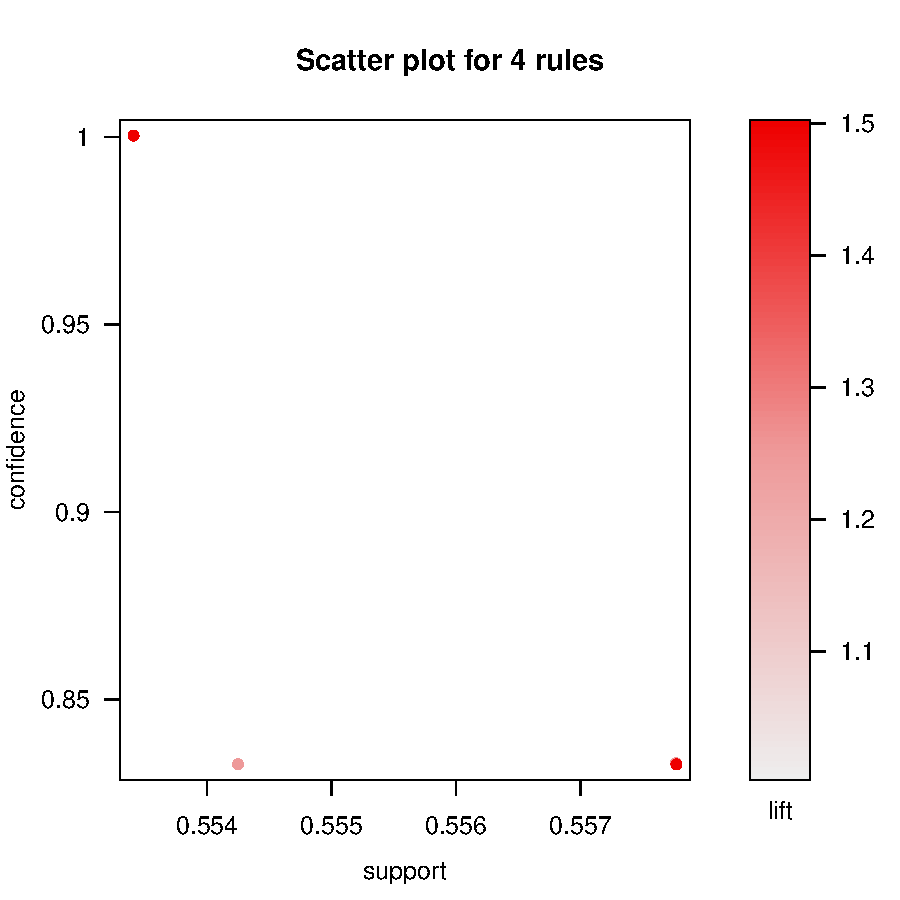
\includegraphics{Memoria-Figura 8}

\section{Análisis de asociación de compras en tecnología}
En esta sección se llevará a cabo un análisis de asociación sobre cuales son los productos que se compran juntos en una tienda de tecnología.

\subsection{Lectura de datos desde archivo Excel}
Para comenzar creamos la matriz nsparse correspondiente y la transponemos, leyendo los datos desde de un archivo Excel:

\begin{Schunk}
\begin{Sinput}
> datosExcelT<-Matrix(as.matrix(read.xlsx("tecnologia.xlsx", 1))
+ ,byrow=TRUE, sparse=TRUE )
> datosExcelngCMatrixT<-as(datosExcelT,"nsparseMatrix")
> trspDatosExcelngCMatrixT<-t(datosExcelngCMatrixT)
> trspDatosExcelngCMatrixT
\end{Sinput}
\begin{Soutput}
10 x 9 sparse Matrix of class "ngCMatrix"
                              
Ordenador    . | . . . . | . .
TV           | . . . | . | . |
Portatil     . | | . | . . | .
Videoconsola | . . . | . . . |
Impresora    . | . . | . . | .
Auriculares  | | . | | | | | .
Teclado      . | . . | . | . .
Raton        . | . . . . | | .
Telefono     . . . . . | . | .
Tablet       . . . | | . . | .
\end{Soutput}
\end{Schunk}

\subsection{Algoritmo Apriori}
A continuación, creamos las transacciones de la matriz en cuestión y aplicamos el algoritmo a priori y obtendremos las asociaciones que cumplen que su soporte, en este caso, sea mayor o igual a 0.3 y la confianza sea mayor o igual a 0.5.  Tambien se muestra un resumen de información acerca de las transacciones creadas.

\begin{Schunk}
\begin{Sinput}
> transaccionesExcelT<-as(trspDatosExcelngCMatrixT,"transactions")
> summary(transaccionesExcelT)
\end{Sinput}
\begin{Soutput}
transactions as itemMatrix in sparse format with
 9 rows (elements/itemsets/transactions) and
 10 columns (items) and a density of 0.3777778 

most frequent items:
 Auriculares           TV     Portatil Videoconsola    Impresora      (Other) 
           7            4            4            3            3           13 

element (itemset/transaction) length distribution:
sizes
1 2 3 5 6 7 
1 3 1 1 2 1 

   Min. 1st Qu.  Median    Mean 3rd Qu.    Max. 
  1.000   2.000   3.000   3.778   6.000   7.000 

includes extended item information - examples:
     labels
1 Ordenador
2        TV
3  Portatil

includes extended transaction information - examples:
  itemsetID
1         1
2         2
3         3
\end{Soutput}
\begin{Sinput}
> asociacionesExcelT<-apriori(transaccionesExcelT,
+ parameter=list(support=0.3, confidence=0.5))
\end{Sinput}
\begin{Soutput}
Apriori

Parameter specification:
 confidence minval smax arem  aval originalSupport maxtime support minlen
        0.5    0.1    1 none FALSE            TRUE       5     0.3      1
 maxlen target  ext
     10  rules TRUE

Algorithmic control:
 filter tree heap memopt load sort verbose
    0.1 TRUE TRUE  FALSE TRUE    2    TRUE

Absolute minimum support count: 2 

set item appearances ...[0 item(s)] done [0.00s].
set transactions ...[10 item(s), 9 transaction(s)] done [0.00s].
sorting and recoding items ... [8 item(s)] done [0.00s].
creating transaction tree ... done [0.00s].
checking subsets of size 1 2 3 done [0.00s].
writing ... [14 rule(s)] done [0.00s].
creating S4 object  ... done [0.00s].
\end{Soutput}
\begin{Sinput}
> inspect(asociacionesExcelT)
\end{Sinput}
\begin{Soutput}
     lhs                        rhs            support   confidence coverage 
[1]  {}                      => {Auriculares}  0.7777778 0.7777778  1.0000000
[2]  {Videoconsola}          => {TV}           0.3333333 1.0000000  0.3333333
[3]  {TV}                    => {Videoconsola} 0.3333333 0.7500000  0.4444444
[4]  {Tablet}                => {Auriculares}  0.3333333 1.0000000  0.3333333
[5]  {TV}                    => {Auriculares}  0.3333333 0.7500000  0.4444444
[6]  {Raton}                 => {Auriculares}  0.3333333 1.0000000  0.3333333
[7]  {Teclado}               => {Auriculares}  0.3333333 1.0000000  0.3333333
[8]  {Impresora}             => {Portatil}     0.3333333 1.0000000  0.3333333
[9]  {Portatil}              => {Impresora}    0.3333333 0.7500000  0.4444444
[10] {Impresora}             => {Auriculares}  0.3333333 1.0000000  0.3333333
[11] {Portatil}              => {Auriculares}  0.3333333 0.7500000  0.4444444
[12] {Portatil,Impresora}    => {Auriculares}  0.3333333 1.0000000  0.3333333
[13] {Impresora,Auriculares} => {Portatil}     0.3333333 1.0000000  0.3333333
[14] {Portatil,Auriculares}  => {Impresora}    0.3333333 1.0000000  0.3333333
     lift      count
[1]  1.0000000 7    
[2]  2.2500000 3    
[3]  2.2500000 3    
[4]  1.2857143 3    
[5]  0.9642857 3    
[6]  1.2857143 3    
[7]  1.2857143 3    
[8]  2.2500000 3    
[9]  2.2500000 3    
[10] 1.2857143 3    
[11] 0.9642857 3    
[12] 1.2857143 3    
[13] 2.2500000 3    
[14] 3.0000000 3    
\end{Soutput}
\end{Schunk}

\subsection{Algoritmo Eclat}
Como ya se ha visto anteriormente, Eclat es una alternativa a apriori.
Se especifica un soporte de 0.3, se van a leer los datos del archivo Excel:

\begin{Schunk}
\begin{Sinput}
> itemsetsT <- eclat(transaccionesExcelT,parameter = list(supp = 0.3, maxlen = 5))
\end{Sinput}
\begin{Soutput}
Eclat

parameter specification:
 tidLists support minlen maxlen            target  ext
    FALSE     0.3      1      5 frequent itemsets TRUE

algorithmic control:
 sparse sort verbose
      7   -2    TRUE

Absolute minimum support count: 2 

create itemset ... 
set transactions ...[10 item(s), 9 transaction(s)] done [0.00s].
sorting and recoding items ... [8 item(s)] done [0.00s].
creating bit matrix ... [8 row(s), 9 column(s)] done [0.00s].
writing  ... [17 set(s)] done [0.00s].
Creating S4 object  ... done [0.00s].
\end{Soutput}
\begin{Sinput}
> itemsetsT
\end{Sinput}
\begin{Soutput}
set of 17 itemsets 
\end{Soutput}
\end{Schunk}

Finalmente se especifica una confianza del 0.5:
\begin{Schunk}
\begin{Sinput}
> rulesT <- ruleInduction(itemsetsT, transaccionesExcelT, confidence = 0.5)
> inspect(rulesT)
\end{Sinput}
\begin{Soutput}
     lhs                        rhs            support   confidence lift     
[1]  {Videoconsola}          => {TV}           0.3333333 1.00       2.2500000
[2]  {TV}                    => {Videoconsola} 0.3333333 0.75       2.2500000
[3]  {Tablet}                => {Auriculares}  0.3333333 1.00       1.2857143
[4]  {Raton}                 => {Auriculares}  0.3333333 1.00       1.2857143
[5]  {TV}                    => {Auriculares}  0.3333333 0.75       0.9642857
[6]  {Teclado}               => {Auriculares}  0.3333333 1.00       1.2857143
[7]  {Impresora,Auriculares} => {Portatil}     0.3333333 1.00       2.2500000
[8]  {Portatil,Auriculares}  => {Impresora}    0.3333333 1.00       3.0000000
[9]  {Portatil,Impresora}    => {Auriculares}  0.3333333 1.00       1.2857143
[10] {Impresora}             => {Auriculares}  0.3333333 1.00       1.2857143
[11] {Impresora}             => {Portatil}     0.3333333 1.00       2.2500000
[12] {Portatil}              => {Impresora}    0.3333333 0.75       2.2500000
[13] {Portatil}              => {Auriculares}  0.3333333 0.75       0.9642857
     itemset
[1]  1      
[2]  1      
[3]  2      
[4]  3      
[5]  4      
[6]  5      
[7]  6      
[8]  6      
[9]  6      
[10] 7      
[11] 8      
[12] 8      
[13] 9      
\end{Soutput}
\end{Schunk}
\subsection{Representación gráfica de Apriori}
En las siguientes graficas se van a visualizar los datos que se han obtenido anteriormente mediante el algoritmo apriori. Para ello se va hacer uso de la librería arulesViz. En primer lugar se representa un grafo dirigido con las asociaciones:
\newline
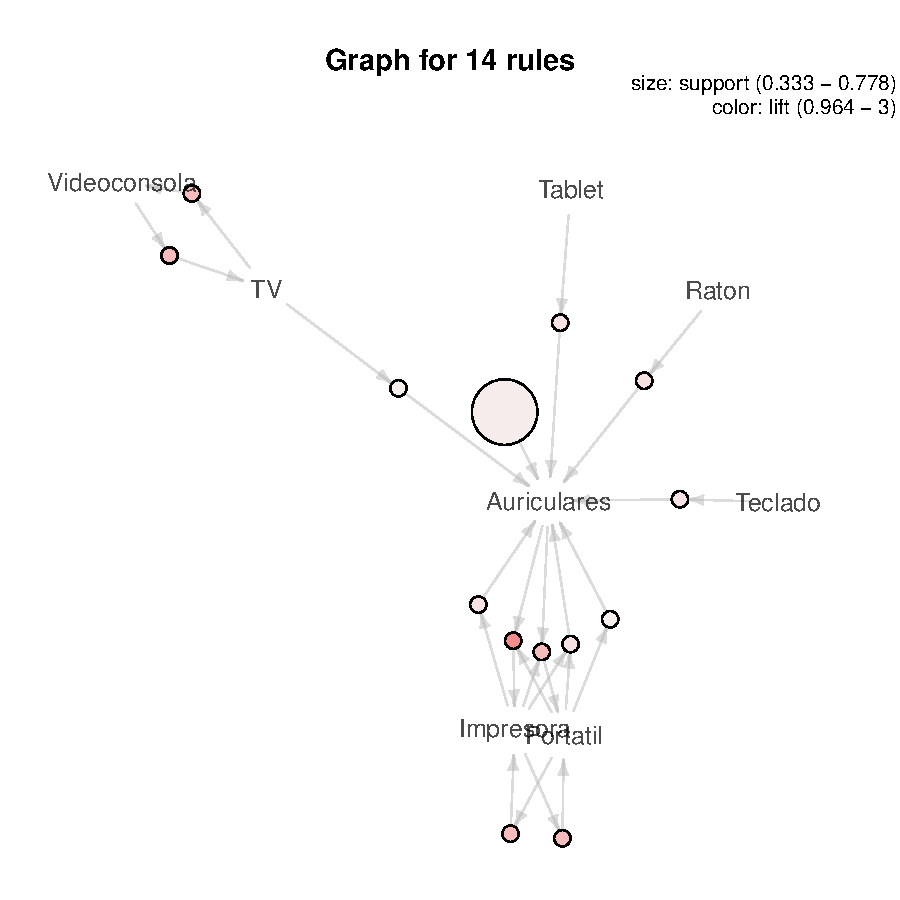
\includegraphics{Memoria-Figura 9}
\newline
A continuación, se va a observar el gráfico disperso, donde cada punto indica una asociación:
\newline
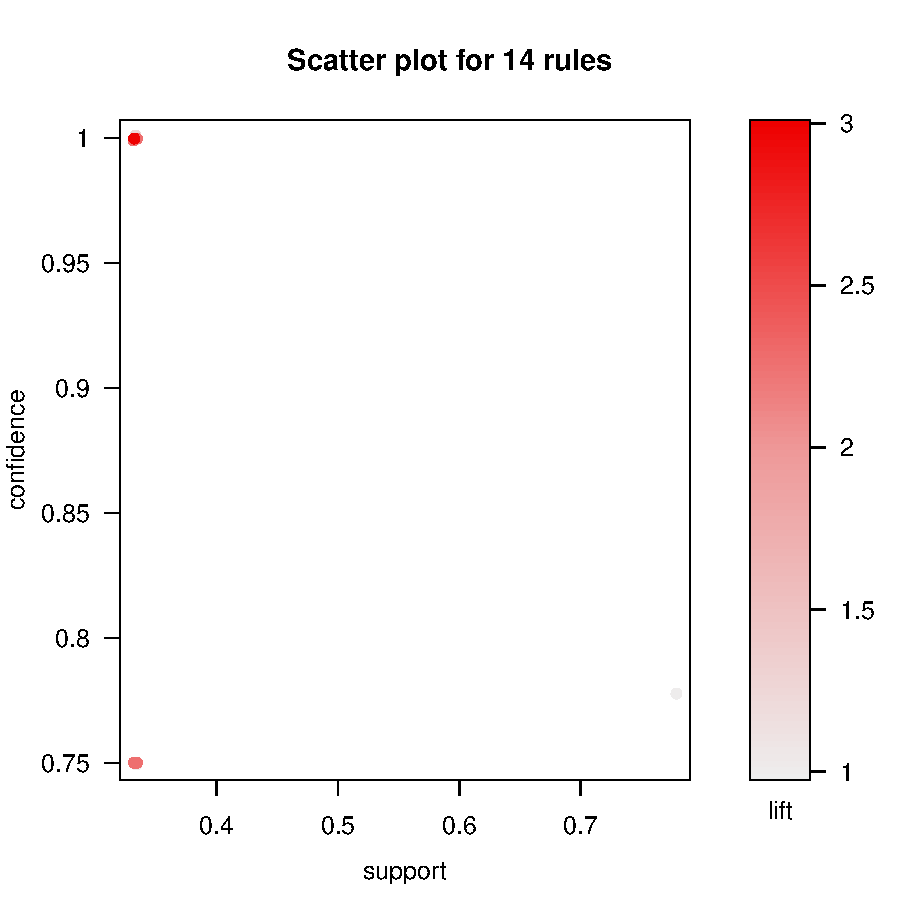
\includegraphics{Memoria-Figura 10}
\newline
\subsection{Representación gráfica de Eclat}
Realizamos las mismas representaciones gráficas realizadas en Apriori para Eclat.
Grafo:
\newline
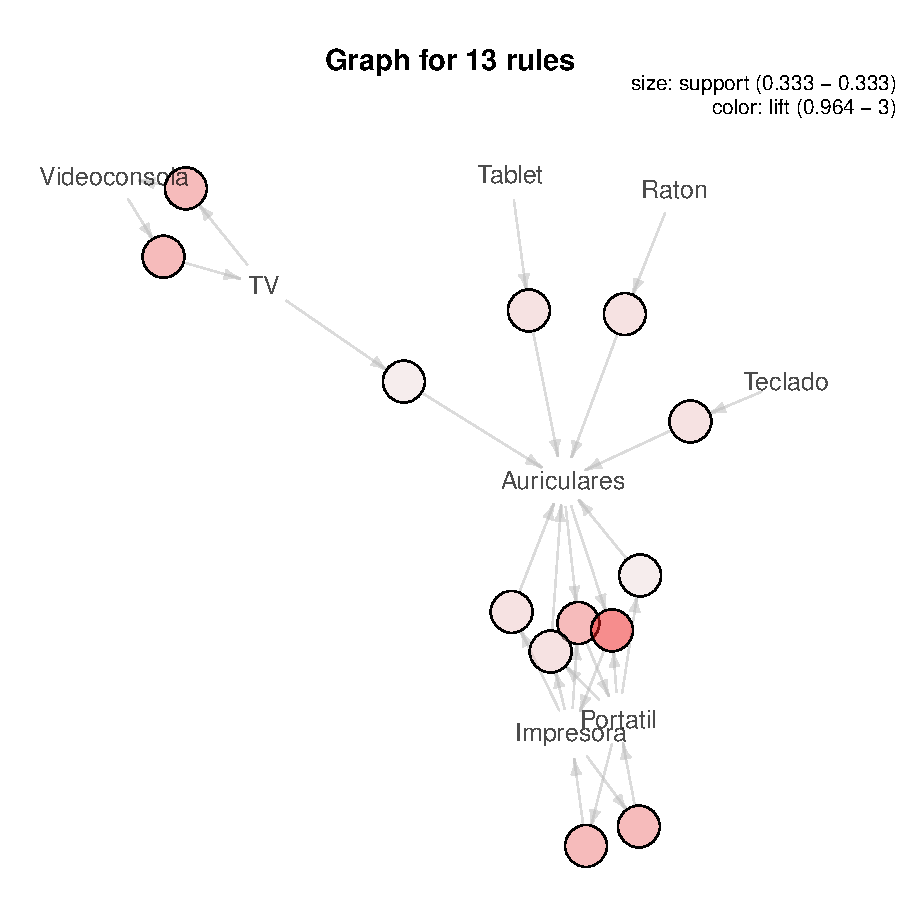
\includegraphics{Memoria-Figura 11}
\newline
Gráfico de puntos dispersos:
\newline
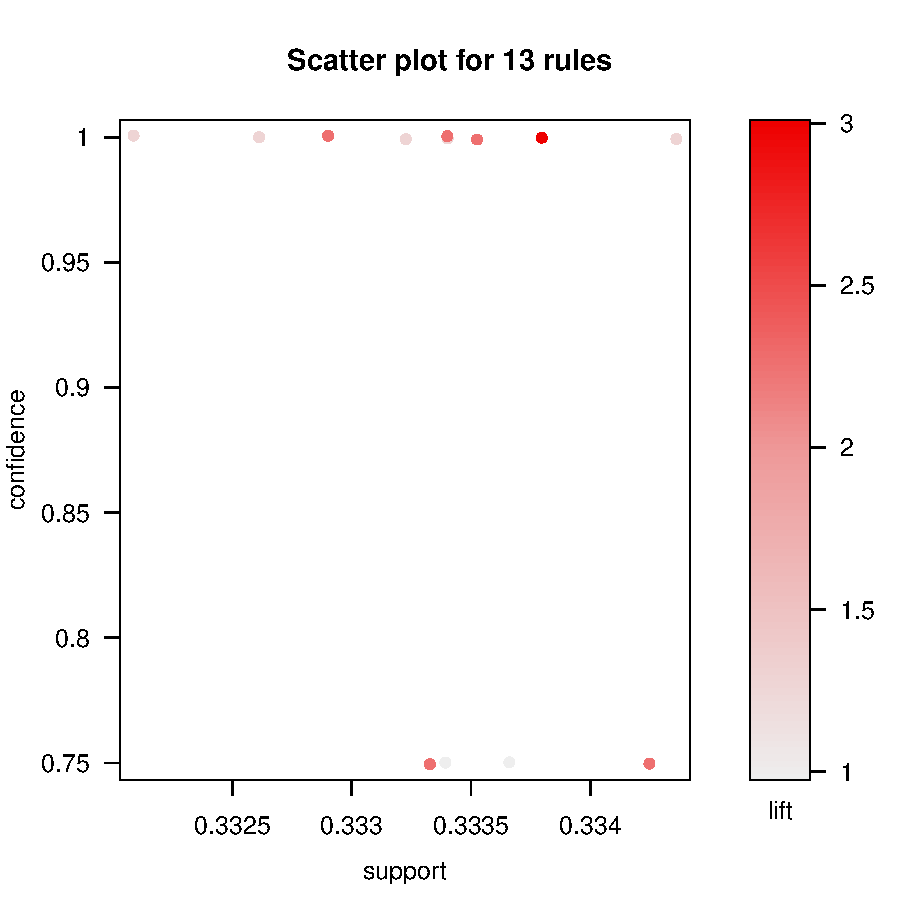
\includegraphics{Memoria-Figura 12}
\newline


\section{Análisis de asociación de compras en papeleria }
En esta sección se realizará un análisis de asociación sobre la compra de productos
en una papelería.

\subsection{Lectura de datos desde archivo Excel}
Para comenzar creamos la matriz nsparse correspondiente y la trasponemos,
leyendo los datos desde de un archivo Excel:

\begin{Schunk}
\begin{Sinput}
> datosExcelP<-Matrix(as.matrix(read.xlsx("papeleria.xlsx", 1)),
+ byrow=TRUE, sparse=TRUE )
> datosExcelngCMatrixP<-as(datosExcelP,"nsparseMatrix")
> trspDatosExcelngCMatrixP<-t(datosExcelngCMatrixP)
> trspDatosExcelngCMatrixP
\end{Sinput}
\begin{Soutput}
10 x 9 sparse Matrix of class "ngCMatrix"
                            
tijeras    . | . . . | . . .
folios     . | . | | | . . .
lapices    . . | | | | . . |
boligrafos | . | . . . | . .
libros     | . . . . | . | .
cuadernos  | . | . . | . . .
borrador   . . | | | | . . |
sacapuntas . . | | | | . . |
compas     . . . . | | . . .
tipex      | . | . . . | . .
\end{Soutput}
\end{Schunk}

\subsection{Algoritmo Apriori}
A continuación, creamos las transacciones de la matriz en cuestión y aplicamos 
el algoritmo a priori y obtendremos las asociaciones que cumplen que su soporte,
en este caso, sea mayor o igual a 0.5 y la confianza sea mayor o igual a 0.8.
Tambien se muestra un resumen de información acerca de las transacciones creadas.

\begin{Schunk}
\begin{Sinput}
> transaccionesExcelP<-as(trspDatosExcelngCMatrixP,"transactions")
> summary(transaccionesExcelP)
\end{Sinput}
\begin{Soutput}
transactions as itemMatrix in sparse format with
 9 rows (elements/itemsets/transactions) and
 10 columns (items) and a density of 0.3888889 

most frequent items:
   lapices   borrador sacapuntas     folios boligrafos    (Other) 
         5          5          5          4          3         13 

element (itemset/transaction) length distribution:
sizes
1 2 3 4 5 6 8 
1 2 1 2 1 1 1 

   Min. 1st Qu.  Median    Mean 3rd Qu.    Max. 
  1.000   2.000   4.000   3.889   5.000   8.000 

includes extended item information - examples:
   labels
1 tijeras
2  folios
3 lapices

includes extended transaction information - examples:
  itemsetID
1         1
2         2
3         3
\end{Soutput}
\begin{Sinput}
> asociacionesExcelP<-apriori(transaccionesExcelP,
+ parameter=list(support=0.5, confidence=0.8))
\end{Sinput}
\begin{Soutput}
Apriori

Parameter specification:
 confidence minval smax arem  aval originalSupport maxtime support minlen
        0.8    0.1    1 none FALSE            TRUE       5     0.5      1
 maxlen target  ext
     10  rules TRUE

Algorithmic control:
 filter tree heap memopt load sort verbose
    0.1 TRUE TRUE  FALSE TRUE    2    TRUE

Absolute minimum support count: 4 

set item appearances ...[0 item(s)] done [0.00s].
set transactions ...[10 item(s), 9 transaction(s)] done [0.00s].
sorting and recoding items ... [3 item(s)] done [0.00s].
creating transaction tree ... done [0.00s].
checking subsets of size 1 2 3 done [0.00s].
writing ... [9 rule(s)] done [0.00s].
creating S4 object  ... done [0.00s].
\end{Soutput}
\begin{Sinput}
> inspect(asociacionesExcelP)
\end{Sinput}
\begin{Soutput}
    lhs                      rhs          support   confidence coverage  lift
[1] {lapices}             => {borrador}   0.5555556 1          0.5555556 1.8 
[2] {borrador}            => {lapices}    0.5555556 1          0.5555556 1.8 
[3] {lapices}             => {sacapuntas} 0.5555556 1          0.5555556 1.8 
[4] {sacapuntas}          => {lapices}    0.5555556 1          0.5555556 1.8 
[5] {borrador}            => {sacapuntas} 0.5555556 1          0.5555556 1.8 
[6] {sacapuntas}          => {borrador}   0.5555556 1          0.5555556 1.8 
[7] {lapices,borrador}    => {sacapuntas} 0.5555556 1          0.5555556 1.8 
[8] {lapices,sacapuntas}  => {borrador}   0.5555556 1          0.5555556 1.8 
[9] {borrador,sacapuntas} => {lapices}    0.5555556 1          0.5555556 1.8 
    count
[1] 5    
[2] 5    
[3] 5    
[4] 5    
[5] 5    
[6] 5    
[7] 5    
[8] 5    
[9] 5    
\end{Soutput}
\end{Schunk}

\subsection{Algoritmo Eclat}

Como ya se ha visto anteriormente, Eclat es una alternativa a apriori.
Se especifica un soporte de 0.5, se van a leer los datos del archivo Excel:


\begin{Schunk}
\begin{Sinput}
> itemsetsP <- eclat(transaccionesExcelP,
+ parameter = list(supp = 0.5, maxlen = 5))
\end{Sinput}
\begin{Soutput}
Eclat

parameter specification:
 tidLists support minlen maxlen            target  ext
    FALSE     0.5      1      5 frequent itemsets TRUE

algorithmic control:
 sparse sort verbose
      7   -2    TRUE

Absolute minimum support count: 4 

create itemset ... 
set transactions ...[10 item(s), 9 transaction(s)] done [0.00s].
sorting and recoding items ... [3 item(s)] done [0.00s].
creating bit matrix ... [3 row(s), 9 column(s)] done [0.00s].
writing  ... [7 set(s)] done [0.00s].
Creating S4 object  ... done [0.00s].
\end{Soutput}
\begin{Sinput}
> itemsetsP
\end{Sinput}
\begin{Soutput}
set of 7 itemsets 
\end{Soutput}
\end{Schunk}

Finalmente se especifica una confianza del 0.5:
\begin{Schunk}
\begin{Sinput}
> rulesP <- ruleInduction(itemsetsP, transaccionesExcelP, confidence = 0.8)
> inspect(rulesP)
\end{Sinput}
\begin{Soutput}
    lhs                      rhs          support   confidence lift itemset
[1] {borrador,sacapuntas} => {lapices}    0.5555556 1          1.8  1      
[2] {lapices,sacapuntas}  => {borrador}   0.5555556 1          1.8  1      
[3] {lapices,borrador}    => {sacapuntas} 0.5555556 1          1.8  1      
[4] {sacapuntas}          => {lapices}    0.5555556 1          1.8  2      
[5] {lapices}             => {sacapuntas} 0.5555556 1          1.8  2      
[6] {sacapuntas}          => {borrador}   0.5555556 1          1.8  3      
[7] {borrador}            => {sacapuntas} 0.5555556 1          1.8  3      
[8] {borrador}            => {lapices}    0.5555556 1          1.8  4      
[9] {lapices}             => {borrador}   0.5555556 1          1.8  4      
\end{Soutput}
\end{Schunk}
\subsection{Representación gráfica de Apriori}
En las siguientes graficas se van a visualizar los datos que se han obtenido
anteriormente mediante el algoritmo apriori.
Para ello se va hacer uso de la librería arulesViz.
En primer lugar se representa un grafo dirigido con las asociaciones:
\newline
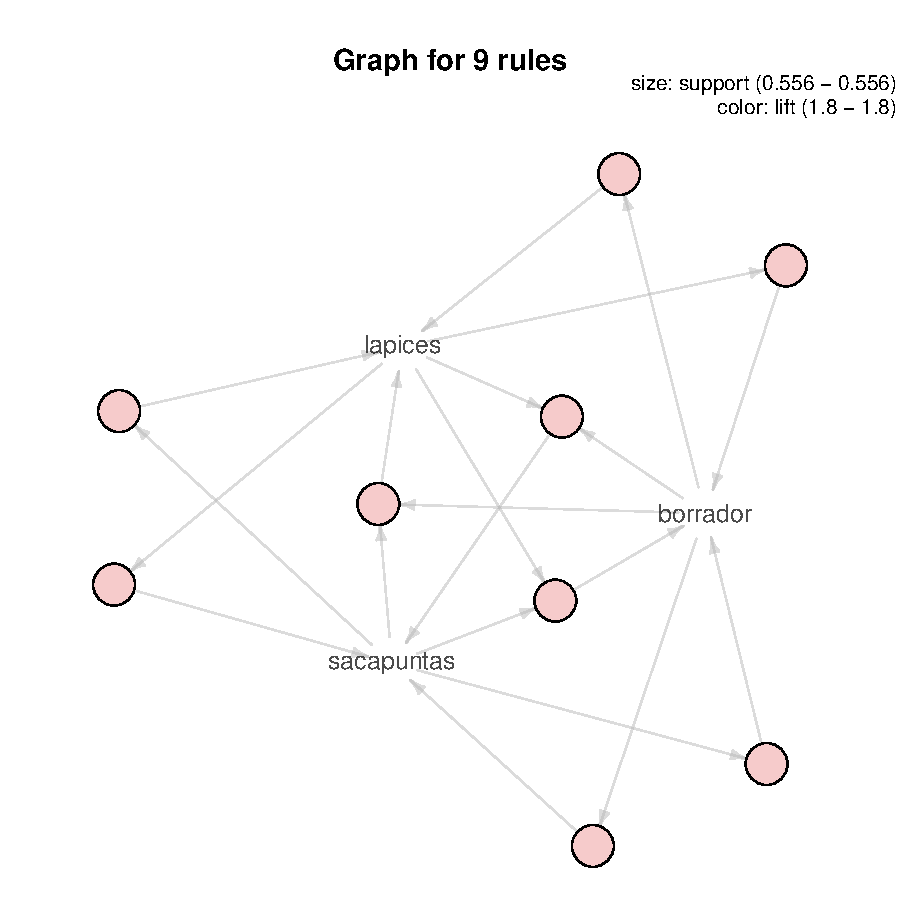
\includegraphics{Memoria-Figura 13}
\newline
A continuación, se va a observar el gráfico disperso,
donde cada punto indica una asociación:
\newline
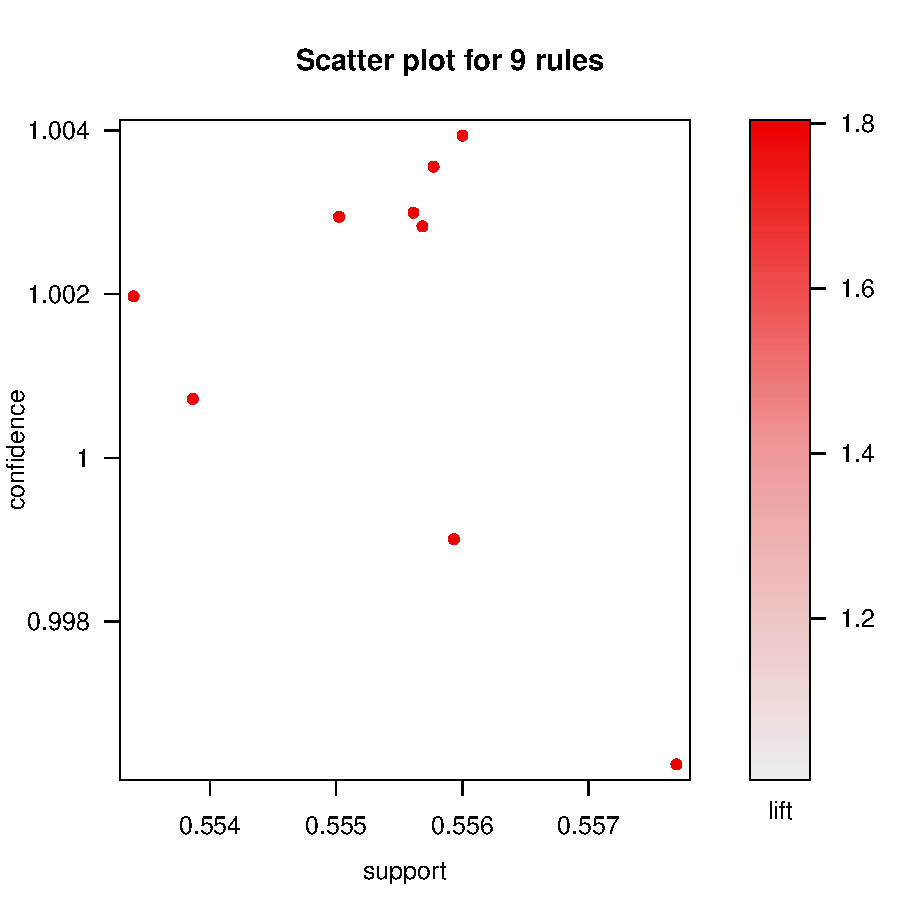
\includegraphics{Memoria-Figura 14}
\newline
\subsection{Representación gráfica de Eclat}
Realizamos las mismas representaciones gráficas realizadas en Apriori para Eclat.
Grafo:
\newline
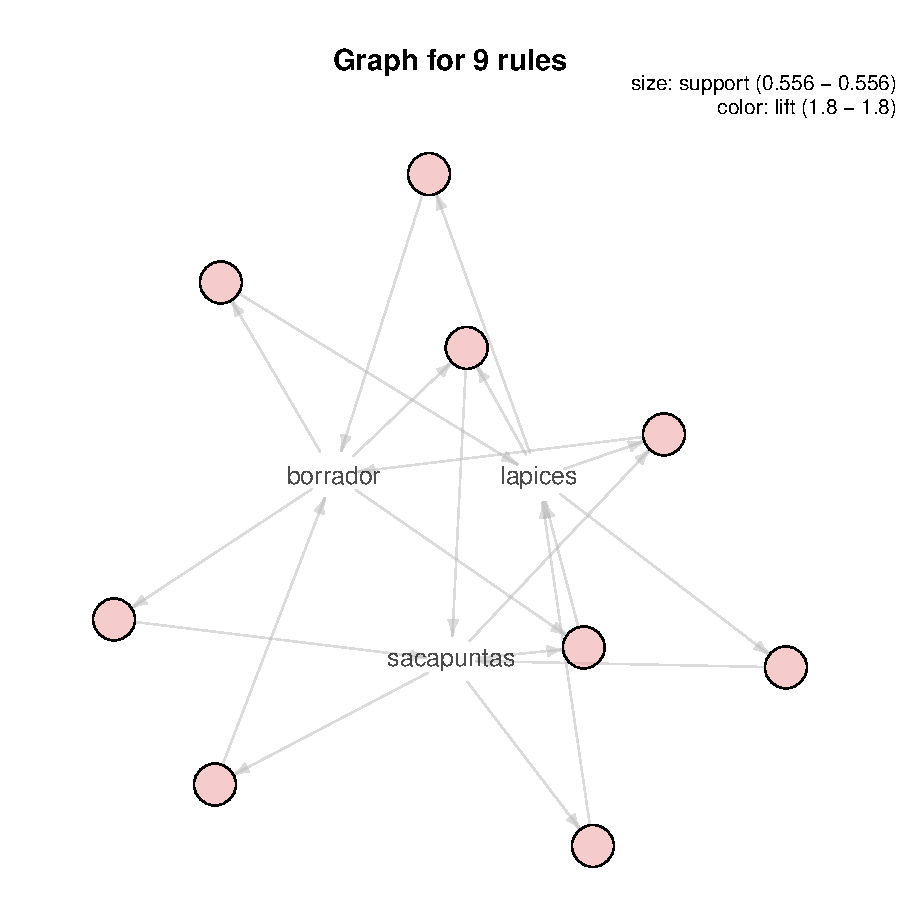
\includegraphics{Memoria-Figura 15}
\newline
Gráfico de puntos dispersos:
\newline
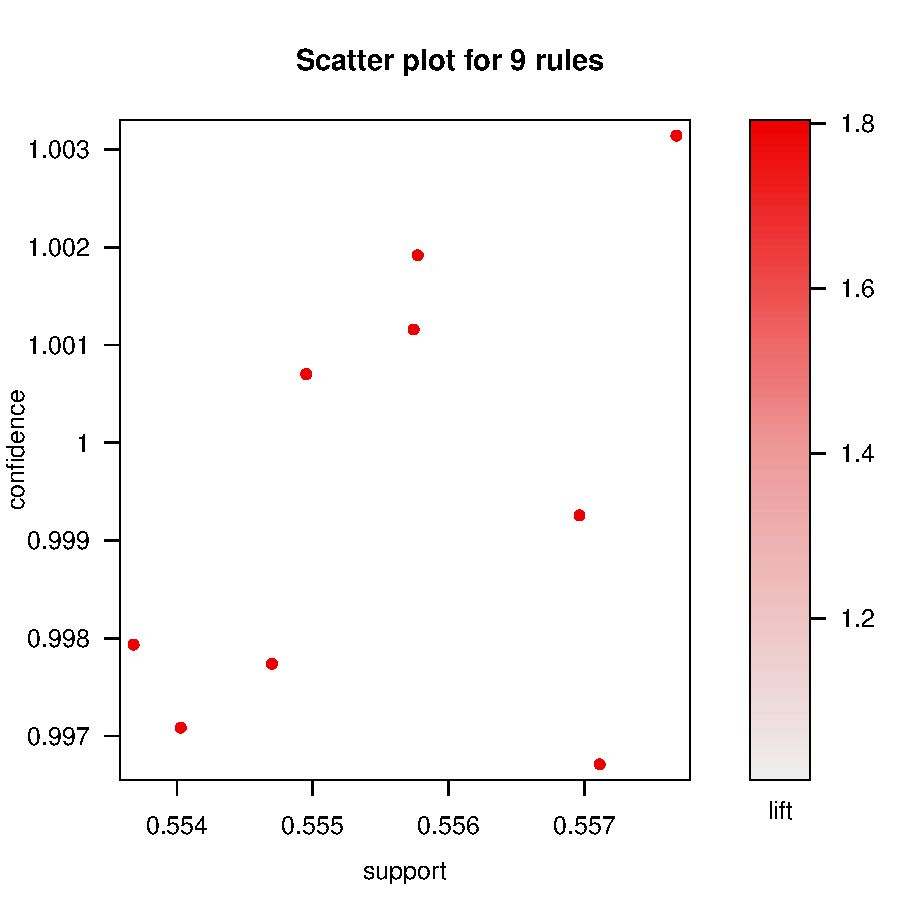
\includegraphics{Memoria-Figura 16}
\newline


\section{Conclusiones}

En esta práctica hemos aprendido a usar en R los algoritmos de asociación. Para su
realización, hemos utilizado el algoritmo visto en teoría (apriori) y hemos añadido
el algoritmo eclat. Estos algoritmos nos permiten averiguar a partir de una muestra
de datos, cuáles son los patrones de aparición conjunta más repetidos
en dicha muestra y que obedecen a unos criterios de soporte y confianza mínimos.
También, al final de cada sección hemos añadido unos gráficos donde se ven las
asociaciones visualmente. Finalmente, tambien cabe mencionar que e  el desarrollo de
esta práctica hemos podido observar como los algoritmos están en constante mejora.
En particular en esta práctica, el algoritmo apriori (que salió el primero) se ha ido
mejorando dando como resultado a mejores algoritmos como el eclat, entre otros.












\end{document}
